\graphicspath{{11-Absorber/Figures/}}

\section{Absorber}
\label{Sect:Absorber}
As a muon beam passes through material, some of the kinetic energy
of the muons is lost through ionization of the material.
This process results in a reduction of the normalised
transverse emittance and the beam is said to be cooled.
Muons will also undergo multiple Coulomb scattering which
increases the divergence of the beam, thereby
increasing the normalised transverse emittance and heating the beam.

Ionization-energy loss is characterised by $\frac{dE}{dx}$, where $E$
is the muon energy and $x$ is the distance travelled within the
absorber.
Multiple Coulomb scattering is characterised by the radiation length,
$X_0$.
For liquid hydrogen, $\frac{dE}{dx} \sim 0.03$\,MeV/mm and $X_0 \sim
8905$\,mm~\cite{PhysRevD.98.030001}.
The absorber vessel was manufactured using aluminium for which
$\frac{dE}{dx} \sim 0.4$\,MeV/mm and $X_0\sim
90$\,mm~\cite{PhysRevD.98.030001}.
To maximise the cooling effect from energy loss in liquid hydrogen,
while minimising the heating effect from multiple Coulomb scattering
in the aluminium windows, these windows were required to be as thin as possible.

Figure~\ref{Fig:AbsorberVessel:Diag} shows the drawings of the absorber focus coil (AFC) module and the installed absorber vessel. The absorber vessel was set at the centre of the FC magnet coils.  Safety considerations required a secondary containment system. Therefore, the absorber vessel was situated in an evacuated space within two more thin aluminium safety windows, so the muon beam had to traverse four windows, as shown in the left panel in Figure~\ref{Fig:AbsorberVessel:Diag}.

geometry definition and validation.

\subsection{Absorber vessel body}
\label{SubSect:AbsorberVessel:Body}

The absorber vessel comprised a cylindrical aluminium body sealed with
two thin aluminium end windows, as shown in the right panel of
figure~\ref{Fig:AbsorberVessel:Diag}.
The absorber vessel was specified to contain 22\,\textit{l} of liquid, so
the body had an inner diameter of 300\,mm and a length between its end
flanges of 230\,mm.  
The length along the central axis between the two domes of the thin aluminium end
windows was 350\,mm.
The body contained an annular cooling channel within its walls
that could act as a heat exchanger. 
This channel was designed to allow the possibility of cooling the
vessel body directly using liquid nitrogen, or even liquid helium. 
However, it was found that this cooling was not necessary because the absorber vessel
cooled sufficiently quickly with cold gas from the condenser,
as described in section~\ref{Sect:Subsect:Helium}. 
Small indium-sealed flanges connected the aluminium pipes from
the absorber vessel to the stainless-steel pipes from the condenser. 

Figure \ref{Fig:AbsorberVessel:BdyPhoto} shows a photograph of the inside of the
absorber vessel body.   
The two flanged windows were sealed to the end flanges of this
body using indium contained in grooves. 
The heat exchanger fins and five pairs of thermometers (LakeShore Cernox 1050-SD)
are visible in this photograph. 
These five thermometer pairs were inside the vessel at locations spaced by 45$^{\circ}$ around
the circumference and were monitored with a LakeShore 218S.
Each pair monitored the presence of liquid hydrogen at that position;
one of these Cernox sensors was operated with a small current as a
thermometer, and the other was occasionally heated by a pulse of larger current.
The difference between the two measured temperatures was small when these sensors
were in liquid due to good cooling efficiency, but the difference was
larger when these sensors were in gas since heat transport through the
gas is worse than in the liquid.
The sensor wires were extracted to vacuum part-way along the
liquid-hydrogen inlet pipe at a 30-pin hermetic feed-through, as
shown in figure~\ref{Fig:AbsorberVessel:Diag}.
Signals from each sensor were carried on two wires inside the absorber
vessel, between the sensor and the feed-through, and by four wires in
the vacuum outside the vessel.
Two Cernox thermometers and two heaters (LakeShore HR-25-100) were
mounted externally on each end flange.
Two additional Cernox
thermometers were mounted externally on the hydrogen inlet and outlet lines.
These thermometers were exposed to vacuum and thermal radiation so the thermometry
here was less accurate than that inside the absorber vessel, but gave indications
of the flow of cooling gas in the circuit. 
To minimise heat input from contact with the magnet bore, the absorber vessel was
mounted on glass-epoxy (G10) supports of low thermal conductivity.
To minimise radiative heat input, multilayer
insulation (MLI) was wrapped around the absorber vessel and all
the low-temperature pipework. 
The number of layers of MLI over the end windows was first entered
into a Monte Carlo program to check that the scattering of muons by
the MLI was insignificant compared to that of the windows, before the
vessel was integrated into the system and cooled.
\begin{figure}
  \begin{center}
    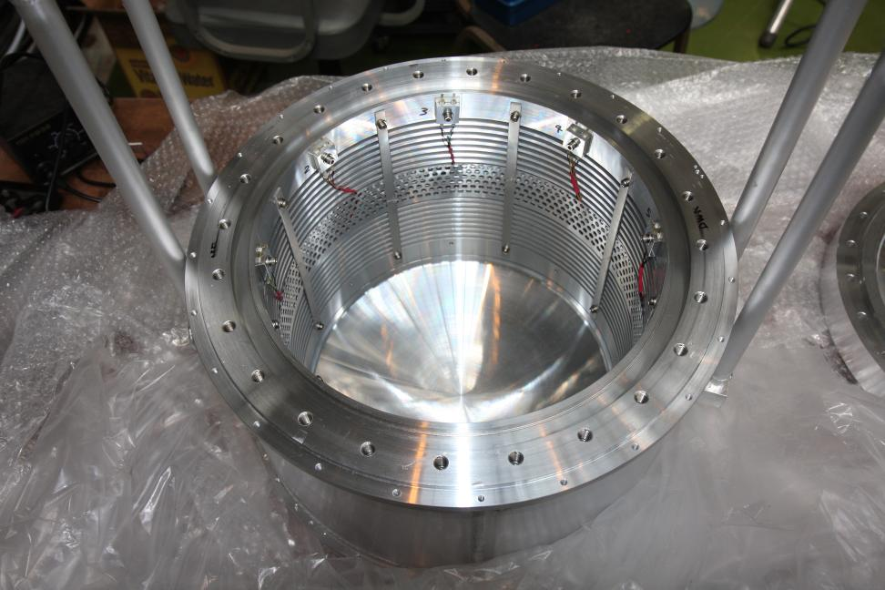
\includegraphics[width=0.95\textwidth]{Abs-Bdy-Photo.pdf}
  \end{center}
  \caption{
    Photograph of the absorber vessel body.
  }
  \label{Fig:AbsorberVessel:BdyPhoto}
\end{figure}

\subsection{Windows}
\label{SubSect:AbsorberVessel:Wndws}

The liquid hydrogen was contained between two aluminium
windows, each having a thickness of 180\,$\mu$m at the centre and
increasing to 360\,$\mu$m near the outer flange. 
Aluminium safety windows, each with a central thickness of 210\,$\mu$m,
enclosed the absorber vessel in the magnet bore.  
Thin aluminium was chosen to minimise multiple scattering.
Thinner windows lead to less scattering
and more muon-beam cooling.
Although a MICE window with a central thickness of 125\,$\mu$m had
successfully been machined using alloy 6061-T651, it  would not withstand
enough pressure. 
The pressure in the absorber vessel reached 1500 mbar during typical operations.
The aluminium alloy we chose to use (6061-T651) was assayed to contain 
 0.61\% silicon, 
 0.26\% iron,
 0.25\% copper,
 0.02\% manganese,
 1.02\% magnesium,
 0.20\% chromium,
 0.01\% zinc, 
 0.05\% titanium,
 0.01\% zirconium, 
 0.15\% maximum other material, 
and at least 97.42\% aluminium (all measured by weight). 
The yield strength was measured at room temperature to be
39,900$\pm$700\,psi (275$\pm$5\,MPa),   
although this would be greater at 20\,K. 
A drawing of a MICE absorber vessel window is shown in
figure~\ref{AbsorberWindow}. 
The double-bend geometry increases the burst strength.

\begin{figure}
  \centerline{\includegraphics*[width=0.99\textwidth]{LH2Absorber2.pdf}}
  \caption{
    Aluminium absorber vessel window with a central thickness of 180 $\mu$m
    for the containment of liquid hydrogen. 
    Both types of safety windows were similar to the vessel window,
  but had a central design thickness of 210\,$\mu$m.
  } 
  \label{AbsorberWindow}
\end{figure}

\subsubsection{Window manufacture}

A CNC Fadal 5020A vertical machining centre and a CNC Romi lathe with
a 27 inch swing were used to machine the windows from a solid block of
aluminium alloy. 
Precision backing plates supported the windows during this process.
Each window was machined to a 2000\,$\mu$m central thickness, and then
measured with the micrometer jig shown in figure~\ref{micrometers}. 
The window was then returned to the lathe for final machining while the
lathe still had the positions stored in its memory.
Clear plastic cases were fabricated to protect the windows from damage
in transit, while still allowing visual inspection.
Finished windows can be seen in figures~\ref{LBL_CMM}
and~\ref{beta_rays}. 

\subsubsection{Window thickness measurement}

The thicknesses of three different types of finished windows
(one absorber and two safety) were measured
with the View Precis 3000 Optical Co-ordinates Measurement Machine
(CMM) shown in figure~\ref{LBL_CMM}.
The complete surface profile of a window was measured with the laser
on one side, and then the window was turned over to measure the other
side.  
The difference between the surface profiles of both sides of the
window gave the thickness.  
Three tuning balls were glued to the window to establish the reference
coordinate system; key to getting a good measurement was to establish
the same reference coordinate system for both sides of each window.
Some results of the measurements are
shown in table~\ref{tab:summary} and figure~\ref{LBL_CMM2}.
For some of the windows, the thickness measurement was checked by
scanning only the small area around the window centre with a very
dense meshing. 
This gave a more accurate measurement of the thickness at the window
centre.

\begin{table}
  \caption{
    Results of measuring the central thickness of the three types of
    windows with the View Precis 3000 Optical CMM shown in
    figure~\ref{LBL_CMM}.
    The windows actually used in MICE were numbers 002, 003, 009, and
    014.
  }
  \label{tab:summary}
  \begin{center}
    \begin{tabular}{|c c c  c c|}
    \hline
Window & Window & Central Thickness & Central Thickness & Note    \rule{0pt}{14pt} \\
 \#  &    Type      & Measured ($\mu$m)              & Design ($\mu$m) &  \\
\hline
001 & Absorber& & 180 & \\
002 & Absorber& $174\pm5$ &180&\\
003 & Absorber& $184\pm2$ & 180&\\
004 & Absorber&& 180&\\
005 & Absorber& $176\pm6$ & 180 &\\
006 & Safety I& $222\pm6$ &210 & flaw at centre\\
007 & Safety I& & 210&  flaw at centre\\
008 & Safety II& $233\pm$5 &210 &\\
009 & Safety II& $230\pm$9 &210 &\\
010 & Absorber&  & 180&\\
011 & Absorber&  & 180&\\
012 & Safety I& $197\pm 7$ & 210  & \\
013& Safety I & & 210  &\\
014 & Safety I & $197\pm8$ & 210 &\\
    \hline
    \end{tabular}
  \end{center}
\end{table}
\begin{figure}
  \begin{minipage}{0.46\textwidth}
    \centerline{\includegraphics*[width=0.9\textwidth]{LBL_measure3}}
    \caption{
      The View Precis 3000 Optical CMM measured the surface profile of
      each window, one side at a time.
    }
    \label{LBL_CMM}
  \end{minipage}\hfill%
  \begin{minipage}{0.46\textwidth}
    \centerline{\includegraphics*[width=0.85\textwidth]{LBL-win003-7B}}
    \caption{
      Result of the CMM measurement of one side of one window. All the axes are
      labelled in units of millimetres.
    }
    \label{LBL_CMM2}
  \end{minipage}
\end{figure}

Low energy electrons are strongly attenuated by modest thicknesses of aluminium. 
Two different beta sources, $^{90}$Sr and $^{204}$Tl, were used to measure the thickness of a MICE
window. The source and detector (Geiger tube) were on opposite sides
of the window so there was no need to 
move the window during this process, as was required with the laser CMM. 
The attenuation of electrons in a thin sheet of material of
thickness $x$ was described using the equation:
\begin{equation}
  R = A \, e^{\,\alpha x} + B\, e^{\,\beta x} + C.
\end{equation}
The apparatus was optimised to measure the central window thickness by
choosing beta sources with electron energies that have a half-range of
about 180\,$\mu$m in aluminium.
Due to electron scattering, the result can be sensitive to apparatus
geometry so a careful calibration was performed using aluminium sheets
of known thickness with
counts being accumulated for 10\,minutes per sheet.
The central thickness of the absorber window in figure~\ref{beta_rays}
was measured to be $178 \pm 6\,{\rm (stat)} \pm 4\,{\rm (fit)}$\,$\mu$m.

\begin{figure}
  \begin{minipage}{0.46\textwidth}
    \centerline{\includegraphics*[height=0.73\linewidth]{micrometer2}}
    \caption{
      Jig for measuring window thickness at the centre and at 15$^{\circ}$
      from the peak of the dome with a pair of
      Starrett T465 micrometers accurate to 3 microns.
    } 
    \label{micrometers}
  \end{minipage}\hfill%
  \begin{minipage}{0.46\textwidth}
    \centerline{\includegraphics*[height=0.73\linewidth]{Beta_window2}}
    \caption{
      $^{90}$Sr and $^{204}$Tl beta sources and a Geiger tube were used to
      check the central thicknesses of windows.
    }
    \label{beta_rays}
  \end{minipage}
\end{figure}
\begin{figure}
  \begin{minipage}{0.46\textwidth}
    \centerline{\includegraphics*[height=0.76\textwidth]{Window_Burst2}}
    \caption{
      This absorber vessel window burst when pressurised with water.
    }  
    \label{Burst_Absorber}
  \end{minipage} \hfill
  \begin{minipage}{0.46\textwidth}
    \centerline{\includegraphics*[height=0.75\textwidth]{Safety_Burst2}}
    \caption{
      This Type I safety window (number 012 in Table \ref{tab:summary})
      burst when slowly pressurised with nitrogen gas.
    } 
    \label{Burst_Safety}
  \end{minipage}
\end{figure}

\subsection{Validation of the absorber model in MAUS}
\label{SubSect:Absorber_Validation}
%% Effect of error in geometry
%%   Test firing particles with modified geometry.
%%   Modified geometry in Scott's analysis.

